\subsection{Posterior Collapse in VCCA-private}
\label{paperB:app:posterior_collapse_in_vcca_private}

We noticed in Table \ref{tab:classification_results_on_test_set} %1 
that VCCA-private achieves similar classification performance as standard VCCA when utilizing the text description $w$ and even worse results when utilizing the iconic image $i$. The private latent variables cannot capture any view-specific variations when each class uses the same iconic image and text description for every natural image. 
A consequence of this is that the iconic image and text description can be identified by only using the shared latent variable $z$ in the decoding phase. The private latent variables are thus not necessary for determining which iconic image or text description to generate, the generated view will be the same anyway for every natural image of a specific class. The model then finds out that the ELBO can be maximized by letting the approximate posteriors be equal to their prior distributions, which minimize the KL divergences of the private latent variables. This phenomenon is referred to as \textit{posterior collapse}~\citeB{B:bowman2015generating}. 

In Figure \ref{fig:kl_divergence_vcca_private} and \ref{fig:kl_divergence_vcca_private_with_iconic_image}, we illustrate that the approximate posterior deduces to its prior distribution -- a zero-mean Gaussian with unit variance -- during training. Figure \ref{fig:kl_divergence_vcca_private}(a) and \ref{fig:kl_divergence_vcca_private}(b) shows the KL divergences over epochs for VCCA-private$_{x w}$ and VCCA-private$_{x w y}$ respectively. The number of words $T=24$ is the same for both models and we train the models for 500 epochs to emphasize that $\KL(q_{\phi_{w}}(u_{w} |w)\,||\,p(u_{w}))$ goes towards zero. We believe that this is due to that there are no variations in the text descriptions within one class (see subsection Investigations of the Learned Representations in Results). We perform a similar experiment with VCCA-private$_{x i}$ and VCCA-private$_{x i y}$ and plot their KL divergences in Figure \ref{fig:kl_divergence_vcca_private_with_iconic_image}. The KL divergence $\KL(q_{\phi_{i}}(u_{i} |w)\,||\,p(u_{i}))$ decreases to zero faster for these models than when we use the text description. We also observe that the KL divergence $\KL(q_{\phi_{x}}(u_{x} |x)\,||\,p(u_{x}))$ decreases to zero as well for both models. Why the KL divergence for the private latent variables decreases faster in the models with the iconic image $i$ is mainly because their likelihood weight $\lambda_{i}$ is smaller than $\lambda_{w}$. We noticed that the KL divergences of the private latent variables decreases slower towards zero when $\lambda_{i}$ is increased, probably because the model foremost focuses on minimizing the reconstruction loss. 

\begin{figure}[t] 
	\centering
	\begin{subfigure}[t]{0.44\textwidth}
		\centering
		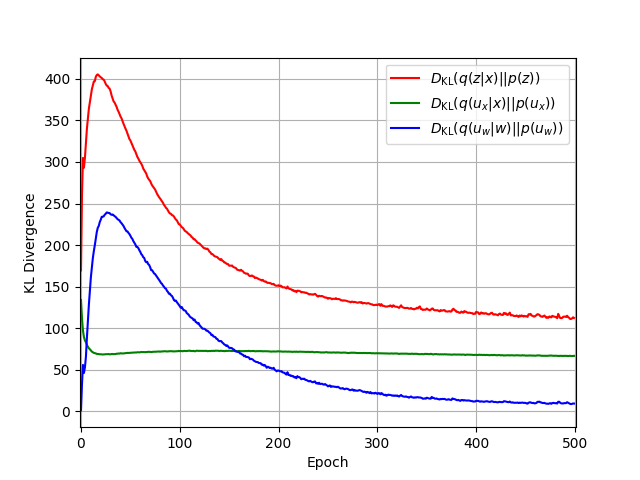
\includegraphics[width=\textwidth]{PaperB/appendix/figures/kl_divergence/kl_vcca_private_xw.png}
		\caption{VCCA-private$_{x w}$}
		\label{subfig:kl_divergence_vcca_private_xw}
	\end{subfigure}~
	\begin{subfigure}[t]{0.44\textwidth}
		\centering
		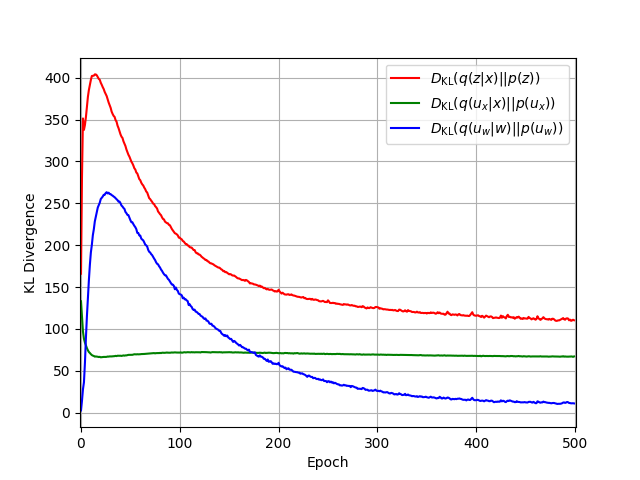
\includegraphics[width=\textwidth]{PaperB/appendix/figures/kl_divergence/kl_vcca_private_xwy.png}
		\caption{VCCA-private$_{x w y}$}
		\label{subfig:kl_divergence_vcca_private_xwy}
	\end{subfigure}
	\caption{The measured KL divergences $\KL(q_{\phi_{z}}(z|x)\,||\,p(z))$ (red), $\KL(q_{\phi_{x}}(u_{x}|x)\,||\,p(u_{x}))$ (green), and $\KL(q_{\phi_{w}}(u_{w} |w)\,||\,p(u_{w}))$ (blue) over epochs. We increased the number of epochs from 200 to 500 to demonstrate that the KL divergence for the private latent variable $u_{w}$ goes to zero. The number of words $T=24$ is the same for both models. The likelihood weights are set to $\lambda_{w} = 1000$ and $\lambda_{y} = 100$. Abbreviations: VCCA, Variational Canonical Correlation Analysis; KL, Kullback-Leibler.
	}
	\label{fig:kl_divergence_vcca_private}
\end{figure}

\begin{figure}[t] 
	\centering
	\begin{subfigure}[t]{0.44\textwidth}
		\centering
		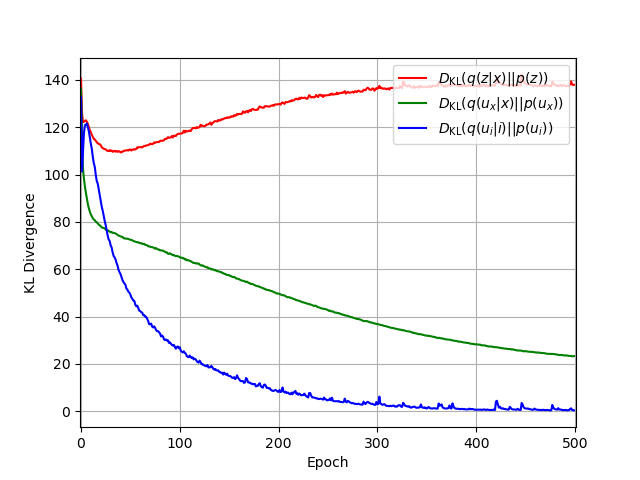
\includegraphics[width=\textwidth]{PaperB/appendix/figures/kl_divergence/kl_div_vcca_private_xi.png}
		\caption{VCCA-private$_{x i}$}
		\label{subfig:kl_divergence_vcca_private_xi}
	\end{subfigure}~
	\begin{subfigure}[t]{0.44\textwidth}
		\centering
		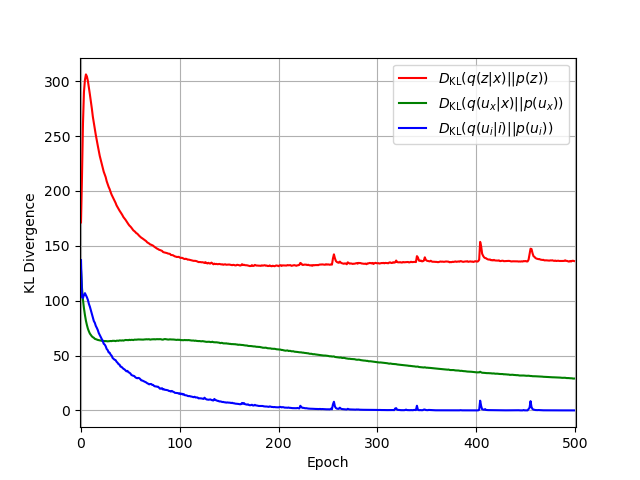
\includegraphics[width=\textwidth]{PaperB/appendix/figures/kl_divergence/kl_div_vcca_private_xiy.png}
		\caption{VCCA-private$_{x i y}$}
		\label{subfig:kl_divergence_vcca_private_xiy}
	\end{subfigure}
	\caption{The measured KL divergences $\KL(q_{\phi_{z}}(z|x)\,||\,p(z))$ (red), $\KL(q_{\phi_{x}}(u_{x}|x)\,||\,p(u_{x}))$ (green), and $\KL(q_{\phi_{i}}(u_{i} |i)\,||\,p(u_{i}))$ (blue) over epochs. We increased the number of epochs from 200 to 500 to demonstrate that the KL divergence for the private latent variable $u_{i}$ goes to zero. The likelihood weights are set to $\lambda_{i} = 10$ and $\lambda_{y} = 1000$. Abbreviations: VCCA, Variational Canonical Correlation Analysis; KL, Kullback-Leibler. 
	}
	\label{fig:kl_divergence_vcca_private_with_iconic_image}
\end{figure}